% Template for a Computer Science Tripos Part II project dissertation
\documentclass[12pt,a4paper,twoside,openright]{report}
\usepackage[pdfborder={0 0 0}]{hyperref}    % turns references into hyperlinks
\usepackage[margin=25mm]{geometry}  % adjusts page layout
\usepackage{graphicx}  % allows inclusion of PDF, PNG and JPG images
\usepackage{verbatim}
\usepackage{docmute}   % only needed to allow inclusion of proposal.tex
\usepackage{listings} % Great for code
\usepackage{color} % Uses color to remind me of things to do.
\lstset{language=Java, showstringspaces=false, basicstyle=\ttfamily\footnotesize, tabsize = 4} % listings settings

\graphicspath{ {figs/} }

\raggedbottom                           % try to avoid widows and orphans
\sloppy
\clubpenalty1000%
\widowpenalty1000%

\renewcommand{\baselinestretch}{1.1}    % adjust line spacing to make
                                        % more readable

\begin{document}

\bibliographystyle{plain}


%%%%%%%%%%%%%%%%%%%%%%%%%%%%%%%%%%%%%%%%%%%%%%%%%%%%%%%%%%%%%%%%%%%%%%%%
% Title


\pagestyle{empty}

\rightline{\LARGE \textbf{Robin McFarland}}

\vspace*{60mm}
\begin{center}
\Huge
\textbf{Giving Programming Exercises Adaptive Difficulty} \\[5mm]
Computer Science Tripos -- Part II \\[5mm]
Homerton College \\[5mm]
2017
\end{center}

%%%%%%%%%%%%%%%%%%%%%%%%%%%%%%%%%%%%%%%%%%%%%%%%%%%%%%%%%%%%%%%%%%%%%%%%%%%%%%
% Proforma, table of contents and list of figures

\pagestyle{plain}

\chapter*{Proforma}

{\large
\begin{tabular}{ll}
Name:               & \bf Robin McFarland                       \\
College:            & \bf Homerton College                     \\
Project Title:      & \bf Giving Programming Exercises Adaptive Difficulty \\
Examination:        & \bf Computer Science Tripos -- Part II, July 2017  \\
Word Count:         & \bf TBC  \\
Project Originator: & Mr Michael B.~Gale                   \\
Supervisor:         & Mr Michael B.~Gale                    \\ 
\end{tabular}
}

\section*{Original Aims of the Project}


\section*{Work Completed}

\section*{Special Difficulties}
 
\newpage
\section*{Declaration}

I, Robin McFarland of Homerton College, being a candidate for Part II of the Computer
Science Tripos, hereby declare
that this dissertation and the work described in it are my own work,
unaided except as may be specified below, and that the dissertation
does not contain material that has already been used to any substantial
extent for a comparable purpose.

\bigskip
\leftline{Signed [signature]}

\medskip
\leftline{Date [date]}

\tableofcontents

\listoffigures

\newpage
\section*{Acknowledgements}

\pagestyle{headings}

\chapter{Introduction}

\chapter{Preparation}

%%%%%%%%%%%%%%%%%%%%%%%%%%%%%%%%%%%%%%%%%%%%%%%%%%%%%%%
% Implementation chapter
\chapter{Implementation}

\textcolor{red}{("it feels a lot like you are explaining the code with the expectation that the reader is looking at the code and reads your description alongside it, when you should really be explaining how it works and what the intuition is (note: explaining how something works is not the same as explaining the code)")}

\textcolor{red}{("You should be approaching the write-up from the perspective of "how do I explain the problems and solutions to someone who has never seen anything about this project before", don't go through the code, pick parts, and describe those.")}

In this chapter I detail the work completed. I begin by describing how I implemented MiniJava, (a small imperative programming language based on Java), as well as a parser for MiniJava's grammar. I then describe the algorithm that allows the addition and removal of ``blanks'' within a MiniJava program. I then describe how a programming exercise is conceptualised in the abstract sense, and give an example of an implementation of a specific question. Finally, I describe the two peripherals I developed to interact with the language; the \texttt{ExerciseSetter} and the Graphical User Interface (GUI).

\section{The Language: MiniJava}

\textcolor{red}{Remove all references to "language features", they are "productions in the abstract syntax".}

In this section I describe how I implemented the MiniJava language.

\begin{figure}
\centering
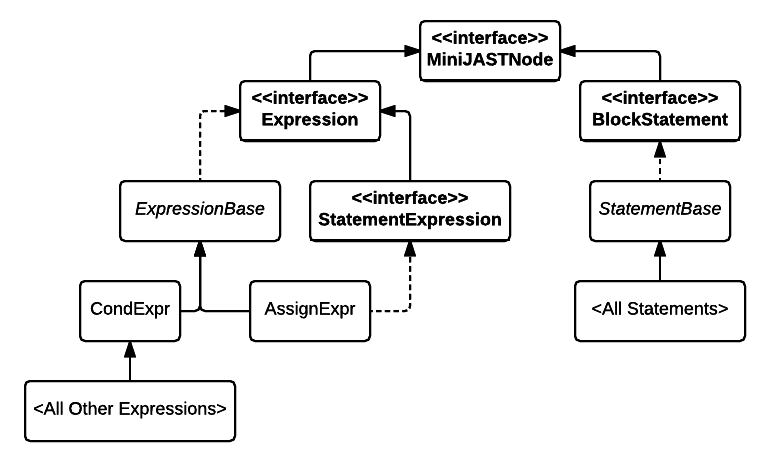
\includegraphics{TopLevelUML}
\caption{The UML diagram showing the top of the object hierarchy for \texttt{MiniJASTNode}s.}
\label{Fig:UML}
\end{figure}

MiniJava is a subset of Java 8 \textcolor{red}{(Fix citation to read [2, p. 714])} (\cite{Java8}  page 714) formed by removing some of the more complex language features, like all object-oriented features. Also, only single-dimensional arrays are allowed. A full description of the grammar of the language can be found in Appendix \ref{App:Parser}. Productions in the abstract syntax of the language have corresponding classes in the implementation. For example, there is a class called \texttt{CondExpr} that corresponds to the production for conditional expressions.. Fig \ref{Fig:UML} shows the top levels of classification that all language features implemented by MiniJava fall into. Ignoring \texttt{MiniJASTNode} for a moment, all language features can be categorised as being either \texttt{Expression} or \texttt{BlockStatements}. Every \texttt{Expression} extends the abstract class \texttt{ExpressionBase}. Some expressions, like \texttt{AssignExpr}, also implement \texttt{StatementExpression}, while others, like \texttt{CondExpr}, do not \textcolor{red}{(Explain the distinction)}. All other expressions extend \texttt{CondExpr}, which gives rise to an implicit operator precedence \textcolor{red}{(Explain this)}. All \texttt{BlockStatements} subclass \texttt{StatementBase}. A MiniJava program can be represented as a tree similar to a parse tree \textcolor{red}{(Make this actually important)}. Thus every class involved needs to implement \texttt{MiniJASTNode} so that operations can be performed on every node of the tree \textcolor{red}{(Explain this better)}. 

Looking at the \texttt{Expression} interface \textcolor{red}{(Either give the code inline or include it in the UML)}, we see the two methods \texttt{evaluate} and \texttt{stringRepr}. The method \texttt{stringRepr} simply returns a \texttt{String} representation of the \texttt{Expression}, evaluated recursively through its sub-nodes. For example: 

\begin{lstlisting}
AddExpr::stringRepr() {
	return leftOperand.stringRepr() + " + " + rightOperand.stringRepr();
}
\end{lstlisting}

\textcolor{red}{(Distinguish between the tree and the interpreter.)}The \texttt{evaluate} method takes a \texttt{Context} object and returns a \texttt{ReturnValues} object \textcolor{red}{(Use bottom explanation, i.e. "The evaluate method implements an interpreter for MiniJava. Before looking at its implementation, let us introduce some helper classes that are needed by the implementation of evaluate.")}. \textcolor{red}{(Give more intuition about what the classes do!)}A \texttt{Context} object stores three maps: \textcolor{red}{(Give the names and then the descriptions)} one map of names to \texttt{Types}, one of names to values, and one of names to depths \textcolor{red}{(Reimplement as Stack-frames!)}. A \texttt{Type} object stores the primitive type (\texttt{boolean}, \texttt{char}, \texttt{int}, or \texttt{double}) associated with the type, and whether the type is an array type or not, and also the size of the type (this is not 1 only if the value is an array). The \texttt{Context} object allows the use of variables. If an identifier has been declared in this scope then it will have an entry in the \texttt{namesToTypes} and \texttt{namesToDepths} maps. If it has also been defined, then it will also have an entry in the \texttt{namesToValues} map. Thus, on variable initialisation, we can check if the identifier has already been used in this scope, and also update its value on assignment. The \texttt{namesToDepths} map is used to keep track of scope, as every time we leave a block (and thus our depth decreases), we remove all the entries from these maps where the depth value is the depth just left.

\textcolor{red}{(Explain intuition)}
\texttt{ReturnValues} is an abstract class, with one implementation for each of the four possible primitive types, and another for an array value. Each of the four implementations stores a value of the appropriate type. \texttt{ReturnValues} objects are how information is passed up the program tree during evaluation. When a node needs to be evaluated, it will evaluate its sub-nodes and use the \texttt{ReturnValues} objects passed up to extract the necessary information. 

\textcolor{red}{(Bottom up explanation)}
Since array accesses are a special case, they require another four implementations of \texttt{ReturnValues} that stores not only the value but also the name of the array it was accessed from and the index it was found at. The reason array accesses require special treatment is that they can be used on the left hand side of assignments. Consider the following code and imagine that array accesses did not get special treatment:

\begin{lstlisting}
a[i++] = i;
\end{lstlisting}

\textcolor{red}{(Explain evaluation better in general)}
In the evaluation of this code, \texttt{a[i++]} is first evaluated as an array access to ensure that \texttt{a} and \texttt{i} are both initialised, and also get the value of \texttt{a[i++]}. Thus the \texttt{ReturnValues} object returned is a \texttt{ReturnValuesInt} that stores the value of \texttt{a[i++]}. The \texttt{i} on the right hand side is then evaluated, and the assignment is ready to take place. \textcolor{red}{(Fluffy, don't use "recognises")}The system recognises that there is an assignment to an array, and attempts to update the value in the \texttt{namesToValues} map, but the system has no way to know what index to store the value at. The \texttt{ReturnValues} object doesn't store it, the \texttt{ArrayAccess} object itself stores it as an \texttt{Expression} which must be evaluated to get a value, which would not only be wrong, but also change the value of \texttt{i} again. Thus there is no way to update an array without having a special version of \texttt{ReturnValues} used for array accesses that also store the index it was meant to be stored at.

Looking now at the \texttt{BlockStatement} interface\textcolor{red}{(Show it again)}, we see the three methods \texttt{execute}, \texttt{executeStart} and \texttt{stringRepr}. In some ways these are analogous to the methods found in the \texttt{Expression} interface. \texttt{stringRepr} returns a \texttt{String} representation of the statement, but also requires a \texttt{blocksDeep} parameter to know how many tab characters to put in front of the text. The \texttt{execute} method takes a \texttt{Context} object and a \texttt{depth} parameter and returns a \texttt{FlowControl} value. The \texttt{depth} parameter is used in scope management by the \texttt{removeDecsAtDepth} method in \texttt{StatementBase}. \texttt{FlowControl} is an enumeration determining what action must be taken after a statement is executed, and can take one of four values: \texttt{BREAK}, \texttt{CONTINUE}, \texttt{RETURN} and \texttt{NONE}. \texttt{executeStart} is simply a helper method for starting an execution with the appropriate initial depth value.

Whenever something goes wrong during execution, for example there is a type error or a variable is used before it is initialised, a custom exception is thrown. Information about the mistake that was made can be extracted from the exception type and from the message passed with it.

In this section I described how the MiniJava language has been designed to allow a program to be stored and executed, and how information can be passed around the program tree.

\section{The Parser}

In this section I explain how a parser for MiniJava was implemented using the ANTLR parser generator \cite{ANTLR4}, and how a MiniJava program tree can be built using it.

\textcolor{red}{("I based the parser grammar on an existing one for Java". Also justify this)}
The GitHub user antlr that owns the antlr4 project containing ANTLR has another project called grammars-v4\footnote{https://github.com/antlr/grammars-v4} that contains lots of example grammars that can be used with ANTLR, including one for Java. I was able to modify this grammar file, in a similar way to how I modified the Java grammar when designing MiniJava, to make a parser generator for MiniJava, \textcolor{red}{(I didn't make a parser generator! A parser generator made my parser to which I added actions)} which can be found in Appendix \ref{App:Parser}. When you \textcolor{red}{(Not you)} use antlr4 on the grammar file, the tool generates a number of files including a \texttt{<GrammarName>BaseVisitor}. By extending this class, one can add actions to the parser. By overriding the appropriate methods in this class, I was able to implement a parser that, given valid MiniJava code, could build a MiniJava program tree. \textcolor{red}{(Talk more about how the parser works)}

\section{The Abstract Question}
\textcolor{red}{(Make title more descriptive, and fix the capitals)}

In this section I explain the formulation of the abstract question and give an example of how a concrete question can be derived from it. \textcolor{red}{(Explain this)}

\textcolor{red}{("The Implementation chapter should not just be a description of every class in your implementation, but an explanation of the key problems you had to solve and how you solved them. From reading your Implementation so far, I have no good idea for why any of these components exist, how they fit together, and what problems they solve.")}

The abstract class \texttt{AbstractPExercise} represents an abstract programming exercise. It has fields including \texttt{question} (a \texttt{String} containing the question shown to students), \texttt{solution} (a \texttt{BlockStatement} object containing the model solution for the problem) and \texttt{baseDifficulty} (a measurement of the relative difficulty of this exercise compared to others, imposes a natural ordering on exercises in terms of their difficulty), and abstract methods including \texttt{setUp} (where the model solution is built) and \texttt{checkSolved} (where the current response is run and the system can determine whether the student has solved the problem). The other fields are required for either actually running the answer, or for adding blanks to and removing blanks from the model solution.

An example implementation of these abstract methods is found in \texttt{FactorialExercise}, \textcolor{red}{(The code won't be provided so if referenced quote it)} an exercise in which the student is asked to use a while loop to calculate the factorial of some integer \texttt{n}, which is supplied on construction of the object. The overridden \texttt{setUp} method constructs the model solution \textcolor{red}{(Explain)}, which represents the code:

\begin{lstlisting}
int total = 1, n = N;
while (n > 1) {
	total *= n--;
}
\end{lstlisting}

where \texttt{N} is the number supplied at construction. This code calculates \texttt{N!} and stores it in \texttt{total} as required. The \texttt{solution} field from \texttt{AbstractPExercise} is filled with the \texttt{Block} object that contains the code. Note also that \texttt{FactorialExercise} defines a new \texttt{totalId} field of type \texttt{Id}, which represents the variable \texttt{total}. This is used in the overriden \texttt{checkSolved} method, where the value of \texttt{total} is checked against the correct answer of \texttt{N!}.

This demonstrates one of the two ways that solutions can be checked: either the value of a variable can be checked by storing its \texttt{Id} in a field and accessing its value later, or an output stream could be printed to using the standard \texttt{System.out.println} method that has been included in MiniJava for convenience and later checked.

In this section I have presented the class \texttt{AbstractPExercise} and given an example implementation of it.

\section{Adding and Removing Blanks}

This section explains the implementation of \texttt{FillableBlank} and its two implementations, before describing the algorithm that adds a blank to a MiniJava program that can later be filled in by a student, and the algorithm that replaces a blank with the original code snippet.

\texttt{FillableBlank} is an abstract class that encapsulates the behaviour of having a unique id and storing the number of nodes that this blank replaces. It is inherited by both \texttt{FillableBlankExpr} and \texttt{FillableBlankStmnt}. \texttt{FillableBlankExpr} implements \texttt{Expression} and \texttt{FillableBlankStmnt} implements \texttt{BlockStatement}, such that both are also \texttt{MiniJASTNodes}. Each stores a \texttt{MiniJASTNode} of the appropriate classification that is either \texttt{null}, or represents student code. 

The algorithm that adds a blank to a MiniJava program is found in the \texttt{addBlank} method of the \texttt{AbstractPExercise} class. The precondition for the algorithm is that the \texttt{solution} field contains a MiniJava program with a certain percentage blank. The postcondition is that either the solution was entirely blank, in which case the algorithm returns false, or the \texttt{solution} field contains the same MiniJava program but with a larger percentage blank, the head of the \texttt{replacedNodes} stack is the replaced node, and the head of the \texttt{replacedNodeTreeIndices} stack is a stack containing the indices describing the path to the blank that has just been added. The increase in percentage blank will be the smallest increment possible at that time.

\begin{figure}[h]
\centering
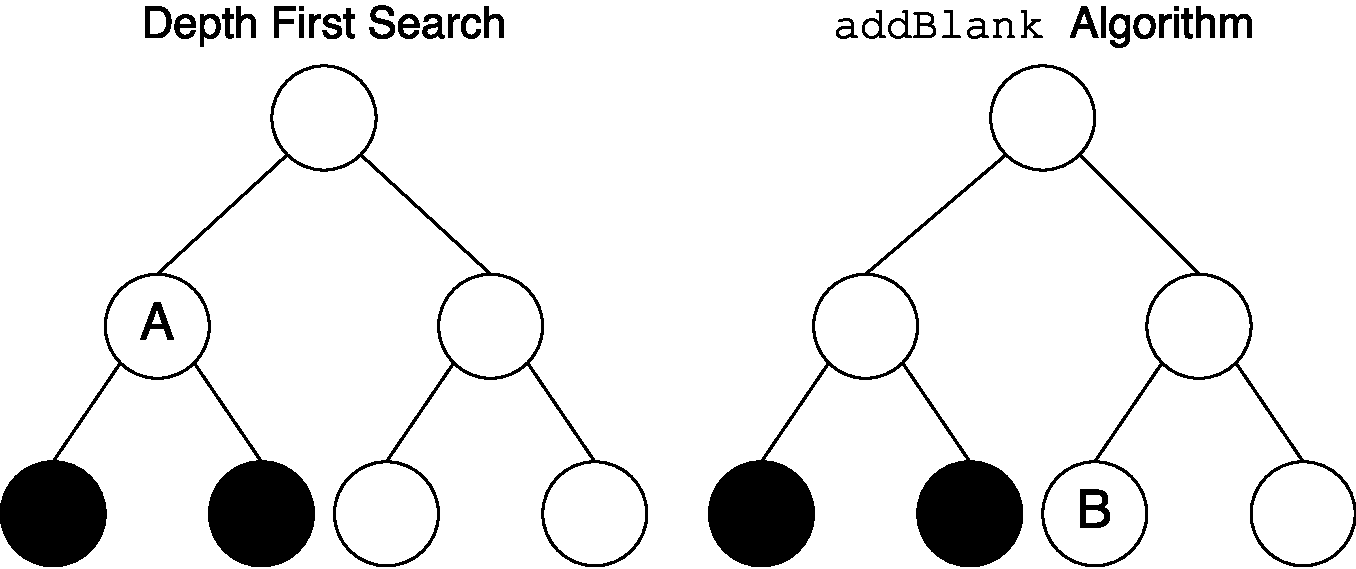
\includegraphics[width=\textwidth]{Searches}
\caption{A figure demonstrating the different behaviour of a depth first search algorithm and my \texttt{addBlank} algorithm.}
\label{Fig:Searches}
\end{figure}
\textcolor{red}{(Reverse Breadth First Search maybe?)}

In order to ensure the increase in percentage blank is the smallest increment possible, the algorithm always selects a leaf to replace with a blank, where here a leaf is defined as a node that either has no children, or all its children are already blank. This desire to reach leaves quickly motivates the use of a depth first search algorithm, but using it without modification presents a problem. Figure \ref{Fig:Searches} shows the difference between the selection made by a depth first search algorithm and the selection that should be made. In the diagram, the black nodes represent blanks, and the white nodes represent nodes in the tree that we might choose to make blank. We see that a normal depth first search algorithm would select node A next, whereas \texttt{addBlank} should select node B. As such, we introduce the notion of ``marking'' a node. When we detect that all of node A's children are blank, we declare that that node is a leaf and we mark it. At this point, the algorithm is looking to replace only unmarked leaves, so on this pass node B will be selected, and on the next pass node A will once again not be selected. Only when all the leaves at this depth have been made blank will node A be made blank.

The nodes are stored in a stack as they are dealt with. However, because more information is required as the algorithm progresses, the parent of the current node being considered, the index of the current node within its parent's \texttt{subnodes} field, and whether the current parent has all its children blank are also stored in stacks. We start by adding the root node of the solution tree to the nodes stack. When we reach a node, it falls in to one of four categories:
\begin{description}
\item[This node's children have already been searched:] {In this case, we need to check whether all of this node's children are blank. If they are, then technically this node is a leaf, but we don't want to replace it next walk of the tree so we mark it accordingly. Either way, we move on to the next node.}
\item[This node is a leaf:]{If this node is marked appropriately, then we need to go about replacing it with a blank. First we will check if this node is in fact the root node, in which case we can replace the entire solution with a blank. Either way, we store the replaced node itself and the path through the tree to its location in terms of indices so that it can later be reinserted if necessary. If the node to be replaced is an \texttt{Expression}, we replace it with a blank expression, otherwise we replace it with a blank statement. Either way we return true, as a replacement has been made.

If instead the node is not marked appropriately, then we move on to the next node after recording that the current parent has a child that is not blank.}
\item[This node is blank:]{If this node is the root of the tree, then the entire solution is blank, and we can't add any more blanks, so we return false. Otherwise, we simply move on to the next node.}
\item[This node is none of the above, and thus has children that need searching:]{In this case we need to register that we are increasing our depth of search. This means we add the current node to the parents stack, we add a new 0 to the indices stack and we add a true to the \texttt{childrenBlank} stack after first recording that the old parent has a child that isn't blank. We then add all this node's children to the nodes stack in reverse order, so that they emerge from the stack in the correct order.}
\end{description}

Within the \texttt{while(true)} loop the entire solution tree is walked. \textcolor{red}{Remove reference to code that can't be seen!)}If a result has not been reached in one iteration of the loop, then all the leaves are marked for not being selected this walk of the tree, so we change the marking we are looking for and walk the solution tree again.

The algorithm that removes a blank from a MiniJava program is found in the \texttt{removeBlank} method of the \texttt{AbstractPExercise} class. It is somewhat simpler than the \texttt{addBlank} method discussed before, as it simply makes use of all the information that has to be recorded during the execution of \texttt{addBlank}. If the \texttt{replacedNodes} stack is empty then there are no blanks to be removed, so we return false. If instead the head of the \texttt{replacedNodeTreeIndices} stack is empty, then we are replacing the whole solution with the head of the \texttt{replacedNodes stack}. Otherwise, we need to follow the path described in the head of the \texttt{replacedNodeTreeIndices} stack (once it has been reversed, since it was stored reversed during \texttt{addBlank}), to find the location of the blank that needs to be replaced by the head of the \texttt{replacedNodes}. We need to make sure that the parent of this node is no longer considered a leaf, and we also need to make sure that if the marking we are searching for was just changed by the last \texttt{addBlank} invocation (i.e. the index we have is always the largest possible) then we change it back now.

This section first explained how the notion of a fillable blank was added to MiniJava, before describing the implementations of the algorithms that introduce them to and remove them from a MiniJava program.

\section{The \texttt{ExerciseSetter}}

In this section I describe how I made use of the language and its features to design the \texttt{ExerciseSetter}, one possible way in which students might interface with exercises designed to facilitate the learning of MiniJava.

The \texttt{ExerciseSetter} stores a list of possible exercises in order of increasing difficulty. The initial exercise to be delivered can be easily adjusted by changing the field \texttt{INITIAL\char`_EX}, and the current exercise index is also stored, along with a reference to that exercise. To measure the difficulty of the exercise and the performance of the students, the number of attempts at a solution made, the number of nodes in the solution, and the number of blanks added are also stored. A lot of the code in this class goes toward keeping these values consistent. The \texttt{ExerciseSetter} also stores a reference to an \texttt{OutputStream}, where all the output can be written to. This allows the \texttt{ExerciseSetter} to be plugged in to other peripherals, like the GUI described below. Finally, it also stores a reference to the parser.

A lot of the methods in this class are helper methods, simply passing messages between the exercise and the student. The important ones are \texttt{fillBlank}, \texttt{reportPerformance}, and \texttt{adjustQuestion}.

\texttt{fillBlank} has two method signatures, one that takes a \texttt{MiniJASTNode}, and one that takes a \texttt{String}. The one that takes a \texttt{MiniJASTNode} is trivial and thus unimportant, but the one that takes a \texttt{String} is more interesting. This method makes use of the parser in an interesting way, as there is of course some ambiguity in the language. The specific ambiguity comes from certain code snippets having the potential to be both \texttt{Expression}s and \texttt{BlockStatement}s. An example of this is the code snippet \texttt{total = 1}. This can be parsed as an assignment, and would thus be classed an \texttt{Expression}, or a variable declaration, where the surrounding context might be \texttt{int total = 1;}, which would categorise this snippet as a \texttt{BlockStatement}. To make the decision, the \texttt{ExerciseSetter} first checks if the blank being filled represents an \texttt{Expression} or a \texttt{BlockStatement}, and sets the entry point for the parser appropriately.

\texttt{reportPerformance} is a possible implementation of a performance heuristic. Performance is based on the number of attempts the exercise took to solve, and the number of nodes in the solution compared with the model solution. The more attempts required and the more nodes in the solution, the worse the performance. A negative result here indicates that the next exercise should be easier, while a positive result indicates it should be harder.

\texttt{adjustQuestion} is a possible implementation of how the performance might influence the difficulty of the next problem. If the next exercise needs to be harder, then the \texttt{ExerciseSetter} adds blanks to the solution until either the exercise is hard enough, or the entire solution is blank. If the latter occurs, then the \texttt{ExerciseSetter} attempts to present a harder problem, and calculate how much of it should be blank. If instead the exercise needs to be easier, then the \texttt{ExerciseSetter} removes blanks from the solution until either the exercise is easy enough, or there are no blanks in the solution. If the latter occurs, then the \texttt{ExerciseSetter} attempts to present an easier problem and calculates how much of it should be blank.

In this section I have detailed one of the ways that students might interface with MiniJava through the \texttt{ExerciseSetter}. This is only an example of a possible use for the tools, but shows how powerful they can be.

\section{The GUI}

In this section I describe the implementation and function of the GUI peripheral.

\begin{figure}[h]
\centering
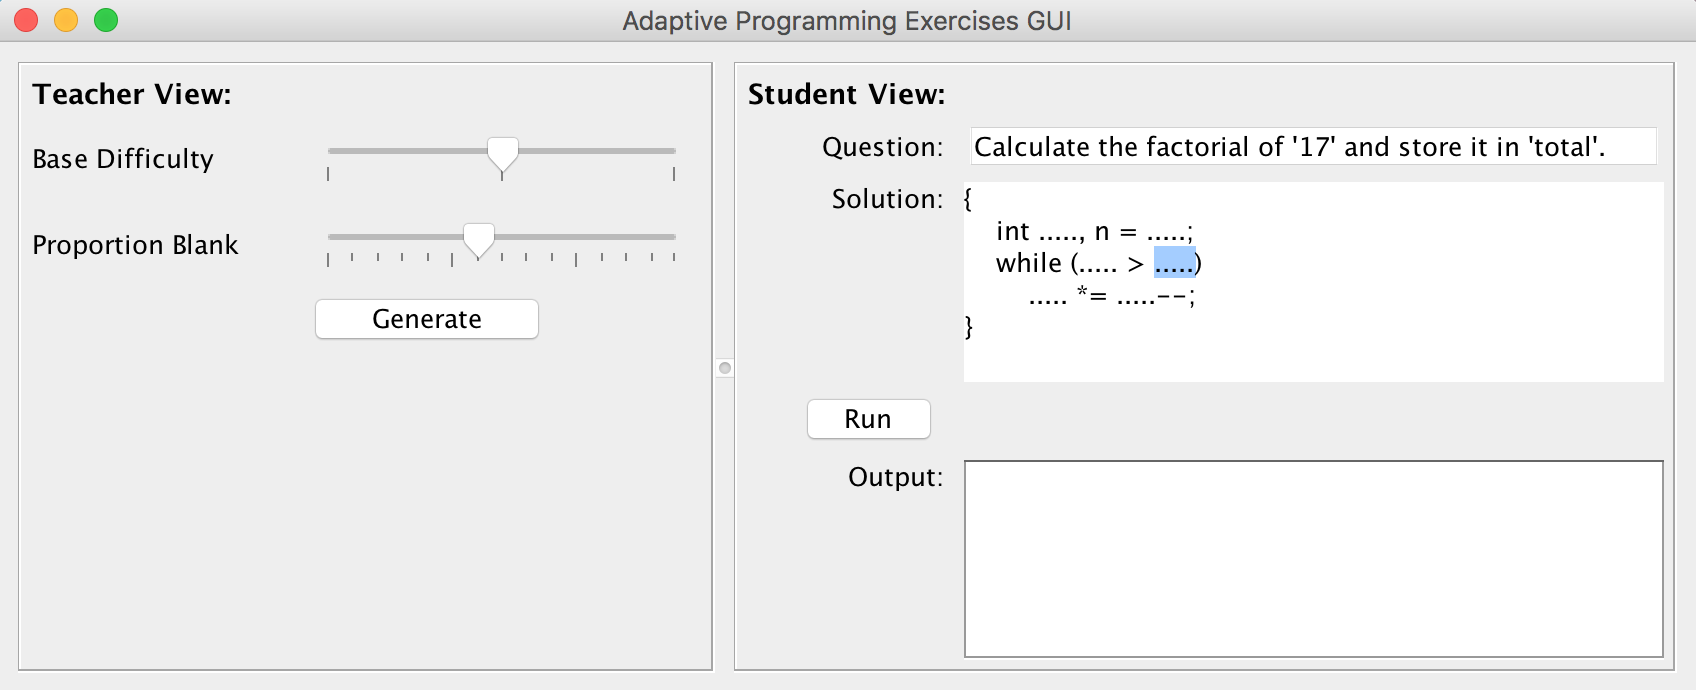
\includegraphics[width = \textwidth]{GUI}
\caption{An example screenshot taken of the GUI peripheral.}
\label{Fig:GUI}
\end{figure}

\textcolor{red}{Make the GUI textbox on the right editable!}

The GUI demonstrates some of the possible uses of this set of tools. It shows how a teacher might manually set the difficulty of a particular exercise and how a student could fill in the blanks and run their solution. An example screen from the GUI is shown in Fig 3. The top slider determines the problem that is presented: the further to the left the slider is, the easier the problem will be. The bottom slider affects the difficulty of that problem: the further it is to the left, the fewer blanks there will be and thus the easier the problem will be to solve. When the ``Generate'' button is pressed, the corresponding exercise will be displayed in the box on the right. 

When an exercise is generated, the blanks within the solution that need to be filled are shown as numbers in brackets surrounded by ellipses. To fill one of the blanks, the user must enter its number in the spinbox, and then enter the code with which to fill the blank in the text box, before pressing the button marked ``Fill Blank''. A blank with a given number can be emptied by entering its number into the spinbox and pressing the button marked ``Empty Blank''. The solution, i.e. the text in the large box on the right, can be executed at any time by pressing the ``Run'' button. The GUI will report whether the solution is correct or not.

The GUI was designed using the IntelliJ UI Designer plugin\footnote{https://www.jetbrains.com/help/idea/2017.1/swing-designing-gui.html}. This plugin allowed me to drag and drop components into place on the form before programming their functionality with the adjoining bound class. The class stores a reference to an \texttt{ExerciseSetter} object, which is where all the data comes from, and where the commands from the user are delivered to. It also makes use of the \texttt{ExerciseSetter}'s \texttt{setOutput} method by giving it a \texttt{ByteArrayOutputStream} that can then be read as text to be displayed. There is some error handling involved in that when something goes wrong, e.g. the user attempts to fill a blank with a number that isn't in the solution, or a solution run raises an error, the error is propagated up from the \texttt{ExerciseSetter} and displayed in the GUI.

This section described the function and then the implementation of the GUI peripheral.\\

In this chapter I have described what I have implemented and how I have done it. I started by giving the design of the language MiniJava, explaining some of these choices by introducing the parser and the concept of ``blanks'' within a MiniJava program. From there I explained how a programming exercise is conceptualised in the abstract sense, and gave an example of an implementation of a specific question. I finished by giving two possible uses for the set of tools, the \texttt{ExerciseSetter} and the Graphical User Interface (GUI).

\textcolor{red}{Estimated Word Count: 3765}

\chapter{Evaluation}

\chapter{Conclusion}

%%%%%%%%%%%%%%%%%%%%%%%%%%%%%%%%%%%%%%%%%%%%%%%%%%%%%%%%%%%%%%%%%%%%%
% the bibliography
\addcontentsline{toc}{chapter}{Bibliography}
\bibliography{refs}

%%%%%%%%%%%%%%%%%%%%%%%%%%%%%%%%%%%%%%%%%%%%%%%%%%%%%%%%%%%%%%%%%%%%%
% the appendices
\appendix

\chapter{The Parser}
\label{App:Parser}

\begin{lstlisting}
grammar MiniJava;

// STATEMENTS / BLOCKS

// entry point
entry
	: block [true]			# blockEntry
	| blockStatement+		# blockStatementsEntry
	| statementTop			# statementEntry
	| expression			# expressionEntry
	;									

block [boolean isOuter]
    :   LBRACE blockStatement* RBRACE						
    ;

blockStatement
    :   primitiveType variableDeclarators SEMI	# localVariableDeclaration
    |   statement								# makeStmnt
    | 	variableDeclarator						# makeVarDec
    ;
    
statementTop
	:	statement						# stmnt
	|	statementNSI					# stmntNSI
	;

statement
    :	block [false]									# makeBlock
    |   IF parExpression statement 						# makeIf
    | 	IF parExpression statementNSI ELSE statement	# makeITE
    |   FOR LPAREN forInit? SEMI expression? 
    			SEMI expressionList? RPAREN  statement	# makeFor
    |   WHILE parExpression statement					# makeWhile
    |   statementNTS									# makeStatementNTS
    ;
    
statementNSI
	:  block [false]										# makeBlockNSI
	| IF parExpression statementNSI ELSE statementNSI		# makeITENSI
	| FOR LPAREN forInit? SEMI expression? 
			SEMI expressionList? RPAREN statementNSI 		# makeForNSI
    |   WHILE parExpression statementNSI					# makeWhileNSI
    |	statementNTS										# makeStatementNTSNSI												
    ;
    
statementNTS
	:	DO statement WHILE parExpression SEMI	# makeDo
    |   RETURN SEMI								# return
    |   BREAK SEMI								# break
    |   CONTINUE SEMI							# continue
    |   SEMI									# empty
    |   expressionStatement SEMI				# makeStmntExpr
    ;


forInit
    :   primitiveType variableDeclarators			# forInitLVD
    |   expressionList								# forInitExprs
    ;

// EXPRESSIONS

parExpression
    :   LPAREN expression RPAREN
    ;

expressionList
    :   expression (COMMA expression)*
    ;

expressionStatement
    :   expression
    ;

expression // Most binding comes first!
    :   Identifier												# makeID
    |   expression LBRACK expression RBRACK						# arrayAccess
    |	parExpression											# makeBracketed
    |   literal													# makeLiteral
    |   expression (op=INC | op=DEC)							# postInc
    |   (op=ADD|op=SUB|op=INC|op=DEC) expression				# preIncEtc
    |   BANG expression											# makeNot
    |   expression (op=MUL|op=DIV) expression					# multExpr
    |   expression (op=ADD|op=SUB) expression					# addExpr
    |   expression (op=LE | op=GE | op=GT | op=LT) expression	# relationalExpr
    |   expression (op=EQUAL | op=NOTEQUAL) expression			# eqExpr
    |   expression AND expression								# andExpr
    |   expression OR expression								# orExpr
    |   <assoc=right> expression QUESTION 
    		expression COLON expression							# condExpr
    |	<assoc=right> expression												
        (   op=ASSIGN
        |   op=ADD_ASSIGN
        |   op=SUB_ASSIGN
        |   op=MUL_ASSIGN
        |   op=DIV_ASSIGN
        )
        expression												# assignExpr
    ;
    
// VARIABLES AND LITERALS
    
variableDeclarators
    :   variableDeclarator (COMMA variableDeclarator)*
    ;

variableDeclarator
    :   Identifier LBRACK RBRACK (ASSIGN variableInitializer)? 	# arrayVarDec 
    |	Identifier (ASSIGN variableInitializer)?				# singleVarDec
    ;

variableInitializer 
    :   arrayInitializerValues									# arrayInitVals
    |	arrayInitializerSize									# arrayInitSize
    |   expression												# initExpr
    ;

arrayInitializerValues
    :   LBRACE variableInitializer (COMMA variableInitializer)* (COMMA)? RBRACE	
    ;
    
arrayInitializerSize
	: 	NEW primitiveType LBRACK expression RBRACK
	;

primitiveType
    :   BOOLEAN
    |   CHAR
    |   INT
    |   DOUBLE
    ;

literal
    :   IntegerLiteral 
    |   FloatingPointLiteral 
    |   CharacterLiteral
    |   BooleanLiteral
    ;

// LEXER

// �3.9 Keywords

BOOLEAN       : 'boolean';
BREAK         : 'break';
CHAR          : 'char';
CONTINUE      : 'continue';
DO            : 'do';
DOUBLE        : 'double';
ELSE          : 'else';
FOR           : 'for';
IF            : 'if';
INT           : 'int';
NEW			  : 'new';
RETURN        : 'return';
WHILE         : 'while';

// �3.10.1 Integer Literals
// �3.10.2 Floating-Point Literals
// �3.10.3 Boolean Literals
// �3.10.4 Character Literals
// �3.11 Separators
// Sections removed for clarity

LPAREN          : '(';
RPAREN          : ')';
LBRACE          : '{';
RBRACE          : '}';
LBRACK          : '[';
RBRACK          : ']';
SEMI            : ';';
COMMA           : ',';
DOT             : '.';

// �3.12 Operators

ASSIGN          : '=';
GT              : '>';
LT              : '<';
BANG            : '!';
QUESTION        : '?';
COLON           : ':';
EQUAL           : '==';
LE              : '<=';
GE              : '>=';
NOTEQUAL        : '!=';
AND             : '&&';
OR              : '||';
INC             : '++';
DEC             : '--';
ADD             : '+';
SUB             : '-';
MUL             : '*';
DIV             : '/';

ADD_ASSIGN      : '+=';
SUB_ASSIGN      : '-=';
MUL_ASSIGN      : '*=';
DIV_ASSIGN      : '/=';

// �3.8 Identifiers (must appear after all keywords in the grammar)
//
// Whitespace and comments
//
// Sections removed for clarity
\end{lstlisting}

\chapter{Project Proposal}

% Note: this file can be compiled on its own, but is also included by
% diss.tex (using the docmute.sty package to ignore the preamble)
\documentclass[12pt,a4paper,twoside]{article}
\usepackage[pdfborder={0 0 0}]{hyperref}
\usepackage[margin=25mm]{geometry}
\usepackage{graphicx}
\usepackage{parskip}
\begin{document}

\begin{center}
\Large
Computer Science Tripos -- Part II -- Project Proposal\\[4mm]
\LARGE
A System for Giving Programming Exercises \\Adaptive Difficulty\\[4mm]

\large
R.~J.~McFarland, Homerton College

Originator: M.~B.~Gale

20 October 2016
\end{center}

\vspace{5mm}

\textbf{Project Supervisor:} M.~B.~Gale

\textbf{Director of Studies:} Dr J.~Fawcett

\textbf{Project Overseers:} Dr D.~J.~Greaves  \& Prof J.~G.~Daugman

% Main document

\section*{Introduction}

Different people learn at different speeds, and learn some things more quickly than others. When a group of students are given a set of programming exercises, this typically isn't taken account of. The aim of this project is to design a system that varies the difficulty of a programming exercise depending on how the individual has performed completing previous exercises. 

The difficulty of an exercise can be measured using two metrics: how complex the problem being solved is and how much code the student is expected to write. The system will vary both of these to adapt the difficulty of proposed exercises automatically (i.e. the system will not look for preprogrammed mistakes, but rather interpret the mistakes made and react accordingly). When an exercise is completed to a sufficient standard, a similar exercise will be given, but expecting more code to be written. When the system has determined that the problem has been mastered, a more difficult problem will be presented, requiring less code to be written again.

\section*{Resources required}

I shall use my own Macintosh laptop for the majority of this project. Backup will be to GitHub and to a 5TB hard drive I keep in my room. I shall make use of the Java standard library, as well as the JavaFX library for the graphical user interface element. I require no special resources.

\section*{Starting point}

I am able to program in Java, and have used JavaFX before for the Part IB group project. During my A-Levels I wrote a program to test the maths abilities of Year 4 students, which involved the programmatic generation of various kinds of maths questions.

\section*{Work to be done}

The work for this project can be split up into the following sub-projects:
\begin{enumerate}
\item{A representation of a programming exercise must be coded up to allow the final product to manipulate them.}
\item{A heuristic that measures the difficulty of a given exercise must be chosen and implemented.}
\item{A heuristic that assesses how well a ``student'' has completed an exercise must be chosen and implemented.}
\item{I must devise a system, using the previous three items, that determines which exercise should be given to the student next, as well as how much of the required code is already filled in, based on the student's performance completing previous exercises.}
\item{A Graphical User Interface should be designed to enable a user to manually adjust the content of a given programming exercise.}
\item{In order to test the program, a student will be simulated by creating a system that tells the program what errors were made where and how long the exercise took to be solved, so that the program's response to various stimuli can be measured.}
\end{enumerate}

\section*{Success Criteria}

The project will be considered completed when:
\begin{enumerate}
\item{I have a system that presents the same initial problem to all students.}
\item{The system can determine that code written by the student solves the given problem.}
\item{On registering completion of the exercise, the system will then present a new problem to the student.}
\item{If the student solved this problem with sufficient ease as measured by my performance heuristic, then this new problem will be more difficult, as measured by my difficulty heuristic.}
\item{If the student failed to solve the problem, or took too much time or made too many errors, then the next problem will be easier.}
\item{The system will adjust the difficulty of a given problem in line with the difficulty heuristic by changing the amount of code required to solve the problem, and also the underlying problem being solved.}
\end{enumerate}

\section*{Possible extensions}

\begin{itemize}
\item{This system could be improved such that it identifies which concepts a student is struggling with and adjusts the content of future exercises to encourage learning of these concepts.}
\item{The program could produce a graph of progress against time to motivate learners.}
\item{A simple game that utilises this system could be made, to showcase how the system might be used to teach programming.}
\end{itemize}

\section*{Timetable}

\textbf{24th Oct - 6th Nov:} 
\begin{itemize}
\item{Research adaptive difficulty and see how it has been done before.}
\item{Research how errors in code have been quantified in the past.}
\item{Research where and how simulated users have been designed to test systems.}
\end{itemize}

\textbf{7th Nov - 20th Nov:}
\begin{itemize}
\item{Describe how code that solves an exercise could be split up into discrete sections, and a way to store how well each of those sections was completed.}
\end{itemize}
\underline{Milestones:}
\begin{itemize}
\item{Have a representation of a programming puzzle in Java code.}
\end{itemize}

\textbf{21st Nov - 4th Dec:}
\begin{itemize}
\item{Prototype and compare heuristics to measure the ``difficulty'' of a given programming exercise, based on the difficulty of the goal to be achieved, and how much of the code is presented initially.}
\end{itemize}
\underline{Milestones:}
\begin{itemize}
\item{Select and implement a difficulty heuristic.}
\end{itemize}

\textbf{5th Dec - 18th Dec:}
\begin{itemize}
\item{Prototype and compare heuristics to measure performance, based perhaps on how much time was taken, the number of errors made and the time the solution takes to run.}
\end{itemize}
\underline{Milestones:}
\begin{itemize}
\item{Select and implement a performance heuristic.}
\end{itemize}

\textbf{19th Dec - 1st Jan:}
\begin{itemize}
\item{Slack time over Christmas to catch up if I need to.}
\end{itemize}

\textbf{2nd Jan - 15th Jan:}
\begin{itemize}
\item{Implement a system to adapt the difficulty of the programming exercises by presenting a new, more difficult problem each time an exercise is completed satisfactorily, and presenting an easier one if the student is struggling too much.}
\end{itemize}
\underline{Milestones:}
\begin{itemize}
\item{Have a system that will present a problem to a student, determine that the student has solved the problem with the code they have written, determine if the student found it too easy or too hard, and present the student with a new problem that is either easier or harder respectively.}
\end{itemize}

\textbf{16th Jan - 29th Jan:}
\begin{itemize}
\item{Write Progress Report.}
\item{Improve the system by implementing the concept of changing the amount of code that needs to be written to solve a given problem as another way of affecting its difficulty.}
\end{itemize}
\underline{Milestones:}
\begin{itemize}
\item{Have the system extended such that it may require the student to write more or less code to make more fine grained adjustments to the difficulty of a programming problem.}
\end{itemize}

\textbf{30th Jan - 19th Feb:}
\begin{itemize}
\item{\textbf{3rd Feb:} Submit the Progress Report}
\item{Design a user interface to change the content of the programming exercise to be solved.}
\end{itemize}
\underline{Milestones:}
\begin{itemize}
\item{Have a user interface with controls to determine the exact difficulty of the problem about to be presented.}
\end{itemize}

\textbf{20th Feb - 5th Mar:}
\begin{itemize}
\item{Write unit tests for all units.}
\end{itemize}
\underline{Milestones:}
\begin{itemize}
\item{Have unit tests written for every unit of the code.}
\end{itemize}

\textbf{6th Mar - 19th Mar:}
\begin{itemize}
\item{Test the implementation by simulating a student ``using'' the system by ``solving'' problems with varying success.}
\end{itemize}
\underline{Milestones:}
\begin{itemize}
\item{Have a simulated student that will tell the system what mistakes were made in the code and where, as well as how long it took to solve the problem (along with any other parameters deemed important to measuring the performance of the student), such that the response of my system can be measured against the performance of a student using it.}
\end{itemize}

\textbf{20th Mar - 2nd Apr:}
\begin{itemize}
\item{Slack time for catching up and doing extensions.}
\end{itemize}

\textbf{3rd Apr - 16th Apr:}
\begin{itemize}
\item{Write Introduction and Conclusion (about 2,500 words).}
\item{Write up Proforma (excluding word count), Declaration of Originality, Project Proposal and Cover Sheet.}
\end{itemize}
\underline{Milestones:}
\begin{itemize}
\item{Have the above sections of the dissertation written in draft form.}
\end{itemize}


\textbf{17th Apr - 30th Apr}
\begin{itemize}
\item{Write Preparation and Implementation (about 5000 words).}
\end{itemize}
\underline{Milestones:}
\begin{itemize}
\item{Have the above sections of the dissertation written in draft form.}
\end{itemize}

\textbf{1st May - 14th May}
\begin{itemize}
\item{Write Evaluation (about 2500 words).}
\item{Write Contents Page, finish Bibliography, Appendices and Index as required.}
\item{Fill in word count of Proforma.}
\item{Submit draft to DoS and Supervisor.}
\end{itemize}
\underline{Milestones:}
\begin{itemize}
\item{Have the above sections of the dissertation written in draft form.}
\end{itemize}

\textbf{15th May - 19th May}
\begin{itemize}
\item{Incorporate feedback into dissertation.}
\item{\textbf{19th May:} Submit dissertation.}
\end{itemize}


\end{document}

\end{document}
